% master.tex : master file for the project
% ------------------------------------------------------------------------------
% This is the main file in the project, which collects the contents from all the
% input files (text, images, literature databases, etc.).

% The 'book' class is a document class with many flexible options.
% See https://tex.stackexchange.com/a/36989/118167
\documentclass[11pt,a4paper,twoside,openright,english]{book}

% Some top level variables that are used to automatically input title, authors,
% etc. in the title page and front page.
\def \projecttitle       {RC-Circuits}
\def \projectsubtitle    {Project Subtitle}
\def \projecttheme       {RC-Circuits}
\def \projectdegree      {Mathematics-Technology}  % or Mathematics-Economics/Technology
\def \projectperiod      {Fall Semester 2019}
\def \projectnumber      {P1}
\def \projectgroup       {C.2-5}
\def \projectauthors     {
  Anders Højbak Lysgaard Lauridsen\\
  Dana Alberte Majgaard\\
  Jakob Olsen\\
  Marjan Anwari\\
  Peter Nørgaard\\
  Sigmundur Beck Jensen
  % ...
}
\def \projectsupervisors {
  John Josef Leth\\
  Kristian Hessellund
  % ...
}

% The preamble, i.e. all the settings and commands that go before actual
% document contents, in this template is handled in the single file aaumath.sty,
% which defines a package that can be loaded here with \usepackage.
\usepackage{aaumath}
\usepackage{amsmath}

% All contents of the document go between the \begin and \end commands for the
% 'document' environment.
\begin{document}

% The front matter is not counted in the numbered pages and are instead numbered
% with roman numerals. This consists of, for example, the front page, title
% page, preface, and table of contents.
\frontmatter
% incl/misc/frontpage.tex : document front page
% ------------------------------------------------------------------------------


\begin{titlepage} % Suppresses headers and footers on the title page

	\centering % Centre everything on the title page
	
	\scshape % Use small caps for all text on the title page
	
	\vspace*{\baselineskip} % White space at the top of the page
	
	%------------------------------------------------
	%	Title
	%------------------------------------------------
	
	\rule{\textwidth}{1.6pt}\vspace*{-\baselineskip}\vspace*{2pt} % Thick horizontal rule
	\rule{\textwidth}{0.4pt} % Thin horizontal rule
	
	\vspace{0.75\baselineskip} % Whitespace above the title
	
	{\LARGE RC-CIRCUITS\\~\\\large -SIMULATION OF TECHNOLOGICAL SYSTEMS } % Title
	
	\vspace{0.75\baselineskip} % Whitespace below the title
	
	\rule{\textwidth}{0.4pt}\vspace*{-\baselineskip}\vspace{3.2pt} % Thin horizontal rule
	\rule{\textwidth}{1.6pt} % Thick horizontal rule
	
	\vspace{2\baselineskip} % Whitespace after the title block
	
	%------------------------------------------------
	%	Subtitle
	%------------------------------------------------
	
	\Large Project report\\\large C.2-5% Subtitle or further description
	
	\vspace*{3\baselineskip} % Whitespace under the subtitle
	
	%------------------------------------------------
	%	Editor(s)
	%------------------------------------------------
	\begin{figure}[H]
	\center
	\includegraphics[scale=0.4]{fig/img/nyfront}
	\end{figure}
	\vspace{0.5\baselineskip} % Whitespace before the editors
	
	
	
	\vfill % Whitespace between editor names and publisher logo
	
	%------------------------------------------------
	%	Publisher
	%------------------------------------------------
	
	
	
	\vspace{0.3\baselineskip} % Whitespace under the publisher logo
	
	\large Aalborg university % Publication year
	
	{\large Mathematics technology} % Publisher

\end{titlepage}

% incl/misc/titlepage.tex : project title page
% ------------------------------------------------------------------------------
% The title page is generated by the command \aautitlepage, which is defined in
% /incl/pre/ext/aautitlepage.sty


\pdfbookmark[0]{Title page}{titlepage}
\aautitlepage{
  \projectinfo{
    \projecttitle
  }{
    \projecttheme
  }{
    \projectperiod
  }{
    Group \projectgroup
  }{
    \parbox[t]{\textwidth}{\projectauthors}
  }{
    \parbox[t]{\textwidth}{\projectsupervisors}
  }{
    \today
  }
}{
  \textbf{Dept. of Mathematical Sciences}\\
  Skjernvej 4A\\
  DK-9220 Aalborg Ø\\
  \href{http://math.aau.dk}{http://math.aau.dk}
}{
  The purpose of this project is to construct a mathematical model of the charging and discharging in an RC circuit, and for high-pass/low-pass filters in signal processing. This can be done using differential equations, circuit theory, complex numbers, and the Laplace transform.
}

% incl/misc/contents.tex :
% ------------------------------------------------------------------------------

\pdfbookmark[0]{Contents}{contents}

% The settings in this file are grouped so they only apply here
\begingroup

% Temporarily disable twoside layout to avoid blank pages in this section
\makeatletter
\@twosidefalse
\makeatother

% Put table of contents on its own page (best for a TOC that fits on one page)
\tableofcontents
%\clearpage

% Put the lists on subsequent pages without page breaks
%\let\clearpage\relax
%\listoffigures
%\listoftables
%\listofalgorithms
%\lstlistoflistings

\endgroup


% The main matter is were the bulk of your work goes. Pages and headings have
% arabic numbers.
\mainmatter
\chapter{Introduction}
\section{Problem analysis}
All electronic devices contain electronic circuits. To be more specific, more or less all of them include a resistor-capacitor circuit (RC circuit). Since these circuits are fundamental in signal processing, understanding the concepts behind them are crucial. From simple definitions of current, voltage, resistors and capacitors, many more useful definitions can be derived by using differential equations, complex numbers, and the Laplace transform. The more advanced definitions are helpful when describing the use of circuits. RC circuits are useful when there is too much noise on signals. In this case, it is possible to derive equations that help cut off unwanted frequencies. Cutting off frequencies can be done using high- and low-pass filters. 

% uddybelse når vi er færdige med projektet
\section{Problem statement}
%Where do differential equations appear in RC circuits? How is the Laplace transform useful when analysing differential equations? How can a mathematical model of an RC circuit be simulated and experimentally validated? How can certain noise-heavy frequencies be removed using RC circuits and can this process be automated using Python?

How can an RC circuit be mathematically explained, and can this be simulated and experimentally validated? How can certain noise-heavy frequencies be removed using RC circuits, and how is this described mathematically?
\chapter{Differential equations}

\section{What is a differential equation?}
A differential equation is any equation, which includes a derivative. These equations aren't solved with a number like a algebraic equations. These equations are solved with a function, or rather a class of functions. \\
An algebraic equation would look something like this: $2x+4=12$. This equation could be solved with $x=4$. However, a differential equation would look something like this: $\frac{dy}{dx} = y$. This equation asks "What function is its own derivative?", which, is of course $y=e^x$. \\

\subsection{Examples of differential equations}
Newton's second law states that the force applied to an object, is the product of the mass of the object, and the acceleration resulting from the applied force. This is written as: 
\begin{align*}
	F=ma
\end{align*}
where $F$ is force, $m$ is mass, and $a$ is acceleration. \\
Acceleration is defined as the change in speed over a time interval. Acceleration is then the derivative of speed, with respect to time:
\begin{align}
	a = \frac{dv}{dt}
\end{align}
It also follows that speed is a change in position over time. Meaning that acceleration can be described with the following equation:
\begin{align*}
	a = \frac{dv}{dt} \rightarrow a = \frac{d^2s}{dt^2}
\end{align*}
Here $s$ represents the object's position, meaning that $ds$ is the objects change in position. \\
Thus force can be described as follows:
\begin{align}
	 F = m\frac{d^2s}{dt^2}
\end{align}
\\
The following are a few other examples of differential equations:
\begin{align}
	af''+bf'+cf =& 5\frac{dy}{dx}		\\
	24cos(t)=&\frac{d^3y}{dx^3}			\\
	f(x)=&4f(x) 						
\end{align}

\subsection{The order of a differential equation}
The order of a differential equation, is denoted as the largest degree derivative present in the equation. Equation (2.3) is then a second order differential equation, (2.4) is a third order differential equation, and (2.5) is a first order differential equation.

\subsection{Separable differential equations} \label{SDE}
A separable differential equation is an equation that takes the form:
\begin{align}
	G(y)\frac{dy}{dx}=H(x)
\end{align}
The equation can then be re-written and solved as follows, assuming that the integral exists\footnote{Assume that $dx$ and $dy$ can be manipulated algebraically. }:
\begin{align}
	G(y)dy=&H(x)dx				\\
	\int G(y)dy =& \int H(x)dx
\end{align}
From here the functions would be integrated, as usual.\\
Then $y$ could be isolated, and the integration constant could be found, if there exists an initial condition for the differential equation.
\begin{tcolorbox}[colback=red!5!white,colframe=red!75!black,title=Example] 
What would the solution be to the following differential equation, with the given condition?
\begin{align*}
	\frac{dy}{dx} = 6y^2x, y(1)=\frac{1}{25}
\end{align*}
The first step is to rewrite the equation, such that it follows the form of (2.6):
\begin{align*}
	\frac{1}{y^2}\frac{dy}{dx}=6x
\end{align*}
Then rewrite the equation to fit the form of (2.7), and then integrate both sides the equations:
\begin{align*}
	\frac{1}{y^2}dy=&6x dx				\\
	\int \frac{1}{y^2}dy=&\int 6x dx		\\
	-\frac{1}{y}=&3x^2+c		
\end{align*}
Given the initial condition the integration constant can be found:
\begin{align*}
	-\frac{1}{\frac{1}{25}}=&3\cdot 1^2+c	\\
	c=&-28
\end{align*}
This would mean that y could be isolated, and the equation would be solved in this specific case:
\begin{align*}
	-\frac{1}{y}=&3x^2-28\\
	y=&-\frac{1}{3x^2-28}
\end{align*}
\end{tcolorbox}
\chapter{Basic circuit theory}
Electrical circuits are fundamental building blocks in, more or less, every electronic device you can think of. The simple act of flipping a switch, e.g. to turn on the light, completes an electrical circuit. The purpose of the circuit is to carry electrical current, either in an open or closed circuit. The electrical components in a circuit are typically resistors, capacitors,  switches, and an electrical 	source (a battery, for instance).
\\ 
In this chapter, if a function is assumed constant, it is denoted with capitalization of its original notation. 
\\ 
\\
The different elements of the circuit can be divided into two categories: active and passive. Active elements supply energy to the system, e.g. a battery, whereas passive elements absorb energy, e.g. a light bulb. A circuit with a battery and a bulb can be represented in the following way.
\begin{figure}[H]
\begin{center}
\begin{circuitikz}[american voltages]
\draw
to[battery, battery1=$V_{B}$, color=blue] (0,2)

to[short, -] (2,2)
[short](2,2)

[short] (2,2)
to [lamp, l=$R_{\text{bulb}}$, color=green](2,0)

(0,0) to [short] (2,0);
\end{circuitikz}
\end{center}
\caption{A circuit with a battery and a light bulb}
\label{fig:bulb}
\end{figure} 
\noindent In figure \ref{fig:bulb} the active element is a battery, and the passive element is a light bulb. Charge is transported by the current from the positive terminal of the battery, through to the light bulb. The light bulb absorbs the energy from the charge, which is then transported to the negative terminal of the battery.
\\

\section{Electric charge}
The electrical charge (in coulombs, $C$) in a circuit stems from the negative charge electrons carry. This charge, when moved through a circuit, is what creates a current.   
\section{Current}
Current $(i)$ is the force that moves charge through a circuit. Current can be defined as an amount of charge moved over a time interval. This can be expressed as the following relation: \cite[p.~3]{bcircuit5}
\begin{align}
i(t)=\dfrac{dq(t)}{dt} \Leftrightarrow q(t)=\int i(t)\ dt,\label{I=dq/dt}
\end{align}
where $i(t)$ is the current (in ampere, $A$) at a given time $t$ (in seconds, $s$), and $q(t)$ is the function for charge at a given time $t$. $q(t)$ is measured in coulomb $(C)$.
\\
There exist two types of current: alternating current (AC) and direct current (DC). Per definition, DC is a constant flow of current, while AC alternates (see figure \ref{fig:ACDC}). 
\begin{figure}[H] 
\begin{tikzpicture}
\begin{axis}[ticks=none,
axis lines =center,
xlabel={t},
ylabel={i(t)},
    height=7cm, width=9cm,
    xmin=0, xmax=10, ymin=-2, ymax=2]
\addplot [
    domain=0:10, 
    samples=100, 
    color=red,
]
{1};
\addlegendentry{$DC$}
\addplot [
    domain=0:10, 
    samples=100, 
    color=blue,
    ]
    {sin(\x r)};
\addlegendentry{$AC$}
\end{axis}
\end{tikzpicture}
\caption{Sinusoidal AC, and DC, versus time}
\label{fig:ACDC}
\end{figure}
\noindent
A sinusoidal AC can be described with the function: 
\begin{align}
i\left(t, f, A, \theta\right) =& A\cdot \sin{\left(2\pi ft + \theta\right)}, \nonumber
\\
=& A \cdot \sin{\left(\omega t + \theta\right)}, \label{eq:omega}
\end{align}
where $f$ is frequency (in hertz, $Hz$), which is cycles per second, $\omega = 2\pi f$ (in radians per second, $s^{-1}$), $t$ is time (in seconds, $s$), $A$ is amplitude (in ampere, $A$), and $\theta$ is the phase shift (in radians, unitless).
For ease of understanding, $\omega$ is sometimes used for notation instead of $2\pi f$. $\omega$ is also called the angular frequency of the signal.
Equation \eqref{eq:omega} with and without a phase-shift can be plotted as such:
\begin{figure}[H]
	\centering
	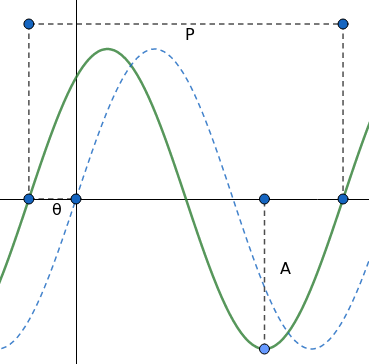
\includegraphics[scale=0.6]{fig/img/AC.png}
	\caption{Two ACs, $i(t)=A\sin(\omega t)$ and $i(t)=A\sin(\omega t+\theta)$ shown in a dotted blue line and a green, respectively. The current shown in green has been phase shifted by $\theta$. The currents have amplitude $A$, and period $P=f^{-1}$.}
\end{figure}
\noindent A certain type of AC exists, where the current is constant for half a period, and then turned off for the other half. This type of AC is called a step voltage, and the graph for this can be seen in figure \ref{fig:AC_step}.
\begin{figure}[H] 
\begin{center}
\begin{tikzpicture}
\begin{axis}[ticks=none,
axis lines =center,
xlabel={t},
ylabel={i(t)},
    height=7cm, width=9cm,
    xmin=0, xmax=10, ymin=-2, ymax=2]
\addplot [
    domain=0:3.14, 
    samples=100, 
    color=red,
]
{1};
\addplot +[mark=none, color=red] coordinates {(3.14, 0) (3.14, 1)};
\addplot [
    domain=3.14:6.28, 
    samples=100, 
    color=red,
    ]
    {0)};
\addplot +[mark=none, color=red] coordinates {(2*3.14, 0) (2*3.14, 1)};
\addplot [
    domain=6.28:9.42, 
    samples=100, 
    color=red,
]
{1};
\addlegendentry{AC step input}
\end{axis}
\end{tikzpicture}
\end{center}
\caption{AC step current versus time}
\label{fig:AC_step}
\end{figure}
\section{Voltage}
Voltage ($v$) is defined as the amount of work that it requires to move a charge of $1 C$ through an element. This is expressed in the following equation: \cite[p. 8]{bcircuit}
\begin{align*}
	v=\dfrac{dw}{dq},
\end{align*}
\\
where $w$ is the work (in watts, $W$).
\section{Resistor}
When a resistor, which is a passive element, is added to a circuit, it creates a resistance ($R$, in ohms, $\Omega$). Resistance makes it more difficult for the current to pass through the element. Resistance is defined as the proportional constant between current and voltage. The mathematical relation of this is given by: \cite[p.~22]{bcircuit5}
\begin{align} 
\label{Ohm}
v(t)=R\cdot i(t),\ R\geq0,
\end{align}
\section{Power} 
Power ($p$) measures energy exerted per second (in watts, $W$). Power can be expressed as: \cite[p. 22]{bcircuit5}.
\begin{align} 
\label{power}
p(t)=v(t)\cdot i(t).
\end{align}
By inserting this in equation \eqref{Ohm}, the following expression is found:
\begin{align}
p(t)=\dfrac{v^2(t)}{R}. \label{resistor:power}
\end{align}

\section{Capacitor}
A capacitor, which is a passive element, consists of two similar sized plates with a distance between them. When a current is applied to the circuit, the capacitor gets charged. The capacitance ($C$) is the amount of energy a capacitor can store, when it is fully charged. The capacitor gets charged, when a positive charge is transferred from one plate to another through the circuit.
\\
The capacitance is given by the following equation:
\begin{align*}
C=\dfrac{\epsilon_{0}A}{d},
\end{align*}
where $C$ is the capacitance (in farad, $F$), and $\epsilon_{0}$ is the permittivity of free space, which is equal to $8.85 \cdot 10^{-12}                                                 \frac{F}{m}$. $A$ is the surface area of the plates (in square meters, $m^{2}$), and $d$ is the distance between the two plates (in meters, $m$).
\\
The charge of a capacitor across a voltage ($v$) and capacitance ($C$) is equal to: \cite[p.~253]{bcircuit5}
\begin{align}
\label{QCV}
q_C(t) = Cv_C(t).	
\end{align}
From \eqref{I=dq/dt}, current is defined as:
\begin{align*}
	i(t) = \frac{dq(t)}{dt}.
\end{align*}
The current across a capacitor is then:
\begin{align*}
	i_C(t) = \frac{d}{dt}\big(Cv_C(t)\big).
\end{align*}
For a capacitor with capacitance ($C$), the current across the capacitor can be written as:
\begin{align}
	i_C(t) = C\frac{dv_C(t)}{dt}.\label{iC}
\end{align}
\section{Time constant}
When describing the charging and discharging of a capacitor, $\tau$ is a useful constant. The product of the resistance ($R$) and the capacitance ($C$) is called the time constant, $R \cdot C = \tau$.

\section{Circuit diagrams}
Electrical circuits are visually represented in circuit diagrams. In addition to the above-mentioned elements, the circuit diagrams introduce three terms: nodes, branches, and loops. Elements are \textit{branches} i.e.  the voltage supply, resistors, capacitors, and the like. \textit{Nodes} connect the \textit{branches} of the circuit. Lastly, any closed path in the circuit, in which no node is encountered more than than once, is called a \textit{loop} \cite[page~32]{bcircuit}. An example of a circuit is shown below.

\begin{figure}[H]
 \begin{center}
\begin{circuitikz}[american voltages]
\draw
to[battery, battery1=$V_{B}$, color=blue] (0,2)
to[resistor, R=$R_1$, color=red] (2,2)
to[resistor, R=$R_2$, color=red] (2,0)
to[short, -] (0,0)
[short, -](2,2) to [short, -] (3,2)
to[resistor, R=$R_3$, color=red](3,0)
to[short, -] (2,0)
[short](3,2) to [short] (5,2)
to [C=$C$, color=green](5,0)
to [short, -] (3,0)
(0,0) to [short, l_=$N_3$, -] (5,0)
(2,2) to [short, l^=$N_2$, -] (5,2)
(0,1) to [short, l^=$N_1$, -] (0,2);
\end{circuitikz}
\end{center}
 \caption{A circuit with a battery, three resistors and a light bulb}
\end{figure}

\noindent This circuit has five branches, which are shown marked in color: a battery (in blue), three resistors ($R_1, R_2,$ and $R_3$, in red), and the light bulb (in green). The three nodes of the circuit ($N_1$, $N_2$, and $N_3$) connect the branches. Additionally, there are three loops, all of which have the same starting and ending point, $V_{battery}$. The first loop passes through $R_2$ and $R_1$, and returns to the starting point. Similarly, the second loop passes through $R_3$ and $R_1$, and returns. The third, and final, loop runs through the light bulb, then $R_1$, and returns. 

\subsection{Kirchhoff's Laws}\label{Klaws}
\textbf{Kirchhoff's Current Law (KCL)}
\\
Observe a circuit up until a node, past which the path of the circuit splits in two. The current encountering the node does not accumulate (as it would e.g. in a battery). Instead, all electrons flowing to that node split up between the available paths, and continue to flow through the circuit. This is Kirchhoff’s current law (KCL), which states that the algebraic sum of all currents in a node is equal to zero. 
\begin{align}
\sum_{j=1}^{N} i_{j}(t) = 0,
\end{align}
where $i_{j}(t)$ is the $j$'th current entering the node through branch $j$, with $N$ branches connected to the node. \cite[page~32]{bcircuit}
\\
\\
\textbf{Kirchoff's Voltage Law (KVL)}
\\
KVL states: In a circuit, the algebraic sum of all voltages in a loop is equal to zero. This can be expressed mathematically  as,
\begin{align}
\sum_{j=1}^{N} v_{j}(t) = 0,
\end{align}
where $v_{j}(t)$ is the voltage in the $j$'th voltage with $N$ voltages.\citep[page~34]{bcircuit}\\



%Example boks
\definecolor{cyan}{RGB}{214,126,120}
\newtcolorbox{definition}{
freelance,
breakable,
before=\par\vspace{2\bigskipamount}\noindent,
after=\par\bigskip,
frame code={
  \node[
  anchor=south west,
  inner xsep=8pt,
  xshift=8pt,
  rounded corners=5pt,
  font=\bfseries\color{white},
  fill=cyan] at (frame.north west) (tit) {\strut Example:};
  \draw[
  line width=3pt,
  rounded corners=5pt,cyan
  ] (tit.west) -| (frame.south west) -- ([xshift=15pt]frame.south west);
},
interior code={},
top=2pt
}

\chapter{Complex Numbers}

\section{Intro}
In the following chapter these sources are used as background information \cite{complexpaul}, \cite{complexpurple}, \cite{complexnotebook}.
When simply using real numbers, you cannot always get the right answer to a given equation. An example of this could be the equation $x^2=-1$. Therefore sometimes we have to use a different number system, which uses the number $i$. 
\begin{align*}
i=\sqrt{-1}
\end{align*}
When squared the number $i$ becomes:
\begin{align*}
i^2=-1
\end{align*}
With the power to the third:
\begin{align*}
i^3=-i
\end{align*}
and with the power to the fourth:
\begin{align*}
i^4=1
\end{align*}
These first four of $i$ creates a loop, $i$ to the fifth will, therefore, be the same as $i$ to the first, $i$ to the seventh is the same as $i$ to the third \\
By using these complex numbers, you can create infinitely more numbers.  
An example of this is the numbers: $2i$ and $-7i$, these are called pure imaginary numbers. When writing pure imaginary numbers you use the form $bi$, where $b$ is a real number that is not $0$. \\
If you put another part on these imaginary numbers, thus $a+bi$ you get the complex numbers. Example $3+4i$ and $-12i+6$. In this case, $a$ is the real part and $b$, where $i$ is, is the imaginary part. $a$ and $b$ are real numbers. By using this method you can make all pure imaginary numbers into a complex number by writing it like this: $0+3i$. $3i$ does not stand alone anymore and is, therefore, a complex number now. You can also rewrite every real number into a complex by doing this $2+0i$. \\
By using complex numbers you can, therefore, find a solution to any given polynomial equation. \\ 
When plotting complex numbers you use the complex plane. The axes are different from the normal coordinate system, instead of the normal $x$ and $y$-axes, you instead have the real part and the imaginary part as the axes. An example of this is shown in the picture below.



\section{Adding and Subtracting}
The rules of addition are much like the rules of simply adding two variables of the same type together. For instance, if you have something like $(5+2i)+(9+8i)$ then you can add the complex numbers and the constants and put it together on the general form; $a+bi$. In this case, we get $14+10i$. This rule can be explained in a general form: 
\begin{align*}
(a + bi) + (c + di) = (a + c) + i(b + d)
\end{align*}
Subtracting is similar because you can only subtract a complex number from another complex number, and the same goes for the constants. Here is an example:
\begin{align*}
(21 + 3i) - (2 - 2i) = 21 + 3i - 2 + 2i = 19 + 5i
\end{align*}
Similarly this can be put in a general form:
\begin{align*}
(a + bi) - (c + di) = (a - c) + i(b - d)
\end{align*}
From the examples above we can see that subtracting and adding with complex numbers is identical to subtracting and adding other and more familiar variables such as ($x$, $y$ so on).

\section{Multiplying}
When multiplying with complex numbers it can get a little different than multiplying with other variables, as $i=sqrt(-1)$ , $i^2=-1$ , $i^3=-i$ , $i^4=1$. \\
\begin{definition}

\begin{align*}
(3+5i)(4-3i) = 12 - 9i + 20i - 15i^2 = 12 + 11i - 15 \cdot (-1) = 27 + 11i
\end{align*}
\end{definition}
The difference is when $x$ is multiplied by $x$ the result is $x^2$, but since there is a definition for $i^2=-1$ the procedure is slightly different. 
This can be described on a general form:
\begin{align}
(a + bi)(c + di) &= a(c + di) + bi(c + di)
&= ac + adi + bci + bdi^2
&= (ac - bd) + i(ad + bc)
\end{align}
Since $i^2 = -1$ then $bdi^2$ can be described as $-bd$.



\section{Dividing}
When dividing with a complex number the aim is to get some values we can put on the general form $a + bi$. 
\begin{definition}

\begin{align*}
\frac{18 + 10i}{3 + 2i} &= \frac{(18 + 10i)(3 - 2i)}{(3+2i)(3-2i)} \\[1em]
&= \frac{54 - 36i + 30i - 20i^2}{9 - 9i^2} \\[1em]
&= \frac{54 - 6i - 20 \cdot (-1)}{9 - 9 \cdot (-1)} \\[1em]
&= \frac{74 - 6i}{9 + 9} \\[1em]
&= \frac{74}{18} - \frac{6}{18}i \\[1em]
&= \frac{37}{9} - \frac{1}{3}i
\end{align*}
\end{definition}
From the example $\frac{37}{9} - \frac{1}{3}i$ is now on the form $a+bi$ with a and b being fractions. In the example the denominator is being conjugated and as a result of that the imaginary part of the denominator $bi$ disappears and is only left in the numerator. 
This can again be described more generally:
\begin{center}
\begin{align*}
\frac{a + bi}{c + di} 										
&= \frac{(a+bi)(c-di)}{(c+di)(c-di)} 						\\[1em]
&= \frac{a(c-di)+bi(c-di)}{a^2+b^2} 							\\[1em]
&= \frac{ac-adi+bci-bdi^2}{a^2+b^2}							\\[1em]
&= \frac{(ac+bd)+i(bc-ad)}{a^2+b^2}							\\[1em]
&= \frac{ac+bd}{a^2+b^2}+i \frac{bc-ad}{a^2+b^2}				
\end{align*}
\end{center}

\section{The Complex Exponential Equation}
The complex exponential equation derives from Euler’s formula, and is necessary to explain the Laplace transformation. \\
%(noget mere tekst)

\definecolor{fersken}{RGB}{236,231,228}
%få den tvunget til at stå på samme side!!!!!!!!!!
\begin{mdframed}[backgroundcolor = fersken,
  frametitle = The Complex Exponential, roundcorner=10pt]
\

 The complex equation of $z=a+ib$ is:
\begin{align}
e^z=e^{a+ib}=e^ae^{ib}=e^a\cos(b)+i\sin(b)
\end{align}
This function has the property:
$$\mid e^{a+ib} \mid = \mid e^x \mid$$
\end{mdframed}


\chapter{Laplace transform}
Up until this point, the project has focused on the behaviour of electrical circuits in the time domain. Observing how different signals change with time yielded a differential equation, as seen in section (\ref{sec371}).
\\ \\
The solution to a differential equation will often be difficult to derive, and this is where the Laplace transform comes in handy. The Laplace transform converts functions of time to functions of frequency (i.e. from the time domain to the \textit{s}-domain). Since the Laplace transform is an integral transform, the rules of integration can also be applied to the Laplace transform.
\begin{definition}{Multiplication by constant}{constant}
If $$ \int c \cdot f(t) \ dt = c \cdot \int f(t) \ dt,$$
then $$\mathcal{L} \left\{c \cdot f(t) \right\} = c \cdot \mathcal{L} \left\{f(t) \right\}$$
\end{definition}
This process reduces the differential equation in question to an algebraic equation. Once the expression has been solved in the \textit{s}-domain, the inverse Laplace transform can be applied to find its corresponding solution in the time domain. Generally, this description can be illustrated in the following way:
\begin{figure}[H]
\center
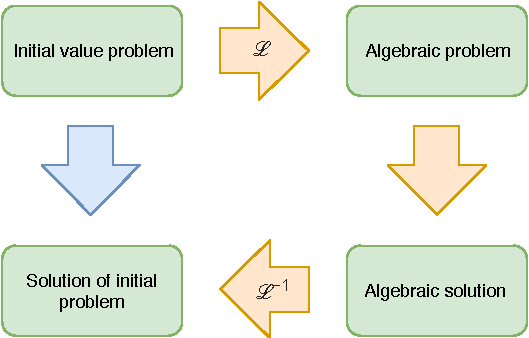
\includegraphics[scale=1]{fig/img/laplace_circ.pdf}
\caption{Solution using Laplace}
\label{lpsol}
\end{figure}

\section{The Laplace Transform}
\begin{definition}{Laplace transform}{lpdef}
\begin{align}
\mathcal{L} \left\{f(t) \right\}=F(s)=\int_{0}^{\infty} e^{-st}\cdot f(t)\ dt
\end{align}
where $f(t)$ is a function of time, $F(s)$ is the Laplace transform of that very function, and $s$ is a complex variable.
\end{definition}
Since the definition consists of an improper integral (integral consisting of infinity), it can be rewritten as:
\begin{align}
\int_{0}^{\infty} e^{-st}\cdot f(t)\ dt = \lim_{N \to \infty} \int_{0}^{N} e^{-st}\cdot f(t)\ dt
\end{align}
When solving something like this, it has to be taken into consideration when the integral converges and diverges. Generally, a function converges when it approaches a specific value. A function diverges when it does not approach a specific value, e.g. when approaching infinity.

\begin{theorem}{Existence of the Laplace transform}{geqleq}

The function $f$ is said to be of exponential order if there exist nonnegative constants $M$, $c$, and $T$  such that $$|f(t)| \leq Me^{ct},$$
which is true for all $t \geq 0$. Thus a function is of exponential order provided that it grows no more rapidly than a constant multiple of some exponential with a linear exponent. \cite[p. 320]{diffandcomplex}
\end{theorem}
\begin{prof}{}{}
Since $f$ is of exponential order, then $|f(t)| \leq Me^{ct}$ for all $t \geq 0$. Note that since $s$ is a complex number  $s=a+ib$, it can be divided into its real and imaginary parts. It then follows that $$\lim_{N \to \infty} \int_{0}^{N} |f(t)e^{-st}|\ dt = \lim_{N \to \infty} \int_{0}^{N} |f(t)| |e^{-ibt}|e^{-at}\ dt$$
By definition \ref{compexpeq}, the complex number $s$ can also take the form: 
$$e^{a}e^{ib}= e^{a}\cos(b)+i\sin(b)$$
Since the imaginary parts are defined as functions of cosine and sine, they can not approach $\infty$. Then naturally $|e^{ibt}|=1$ for all $b \in \mathbb{R}$. This now yields $$\lim_{N \to \infty} \int_{0}^{N} |f(t)e^{-at}|\ dt \leq \lim_{N \to \infty} \int_{0}^{N} Me^{ct}e^{-at}\ dt = M \lim_{N \to \infty} \int_{0}^{N}e^{-(c-a)t}\ dt $$ The integral is only going to converge when $(a-c)>0$ or Re$(s)>c$.
\end{prof}

\begin{example}{Laplace transform for $1$}{lpone}
From definition \ref{lpdef}, let $f(t)=1$. In that case,
\begin{align*}
\mathcal{L}\{f(t)\}=\int_{0}^{\infty} e^{-st} \cdot 1\ dt
\end{align*}
Now $\infty$ is replaced with some value $N$ that is set to approach $\infty$:
\begin{align*}
\mathcal{L} \left\{f(t) \right\}= \lim_{N \to \infty}  \int_{0}^{N} e^{-st}\ dt
\end{align*}
$e^{-st}$ is now integrated with respect to $t$:
\begin{align*}
\mathcal{L} \left\{f(t) \right\}= \lim_{N \to \infty} \left[ -\dfrac{1}{s} e^{-st} \right]_{0}^{N} \ 
\end{align*}
Zero and $N$ is now inserted on $t$’s place:
\begin{align*}
\mathcal{L} \left\{f(t) \right\}= \lim_{N \to \infty} \left( -\dfrac{1}{s} e^{-sN} - \left(-\dfrac{1}{s}\right) \right) \ 
\end{align*}
Now observe what happens when $N$ approaches $\infty$:
\begin{align*}
\mathcal{L} \left\{f(t) \right\}=\dfrac{1}{s} \ \ \ ; \ \ \ Re(s) > 0
\end{align*}
Here the real part of $s$ has to be greater than zero, hence it makes $-\dfrac{1}{se^{sN}}$ converge towards zero. If it is less than zero the expression would start to diverge, and would therefore not make sense to look at.
\end{example}

\begin{example}{Laplace transform for $e^{at}$}{lpe}
From definition \ref{lpdef}, let $f(t)=e^{at}$, where $a$ is a constant, and $t$ is time. In that case,
$$\mathcal{L} \left\{f(t) \right\}=\int_{0}^{\infty} e^{-st}\cdot e^{at}\ dt$$
Since they have the base, $e$, in common, their exponents can be combined. Additionally, $t$ can be factorised:
$$\mathcal{L} \left\{f(t) \right\}=\int_{0}^{\infty} e^{-(s-a)t}\ dt$$
Since it is an improper integral, the limits are applied. This means that some number is set to approach infinity. Here N is set to approach $\infty$:
$$\mathcal{L} \left\{f(t) \right\}=\lim_{N \to \infty} \int_{0}^{N} e^{-(s-a)t}\ dt$$
Integration by substitution is now applied. Let $\dfrac{du}{dt}=-(s-a)$. This yields $dt=-\dfrac{1}{s-a}du$. The integral is now no longer from 0 to $\infty$, since new limits are applied. It is now an integral from $u=-(s-a)0=0$ to $u=-(s-a)N$. Since $-\dfrac{1}{s-a}$ is a constant it can be moved outside the integral. It is going to look like this:
\begin{align}
\mathcal{L}\{f(t)\}=\lim_{N \to \infty} \int_{0}^{-(s-a)N} e^{u}\cdot -\dfrac{1}{s-a}\ du = \lim_{N \to \infty} -\dfrac{1}{s-a} \cdot \left[e^{u} \right]_{0}^{-(s-a)N}
\label{eq6.2}
\end{align}
Now applying $u=0$ and $u=-(s-a)N$ to $e^{u}$:
\begin{align*}
\mathcal{L} \left\{f(t) \right\} =\lim_{N \to \infty} -\dfrac{1}{s-a}\cdot (e^{-(s-a)N}-e^{0})
\end{align*}
Since $e^{-(s-a)N}$ will approach $0$, when $N$ is approaching $\infty$ (if $Re(s) \geq a$). Therefore the equation is going to look as follows:
\begin{align}
\mathcal{L} \left\{f(t) \right\} = \dfrac{1}{s-a}
\end{align}
In conclusion, the Laplace transform of $f(t)=e^{at}$ equals
$$\mathcal{L} \left\{f(t) \right\} =\dfrac{1}{s-a} \ \ \ ;\ \ \ Re(s)>a$$
$s$ must be greater than $a$, since the limit of $e^{-(s-a)N}$ converges towards zero. If $a$ is greater than $s$, the exponent of $e$ would be positive, and the limit would diverge.
\end{example}
%The Laplace transform can be used for all functions of $f$, where the real part of $s$ is greater than $a$ $Re(s) \geq a$. Since $s$ is a complex number ($s=a+ib$), only the first part of $s$ has to be greater than $a$. Therefore, $e^{-st}$ is  the same as $e^{-ta}e^{-tib}$, where the last part is the imaginary part of the complex number. In the complex chapter, this is also defined as $e^{a}\cos(b)+ i \sin(b)$.% 
When doing the inverse Laplace transformation, the results can often be found by looking at the results from on ordinary Laplace transformation.
\begin{example}{Inverse Laplace transform}{}
Let $F(s) = \dfrac{4}{s+10}$. When recognizing this takes the same form as the result above, the solution becomes clear. Now this has to be put on the form $f(t)=e^{at}$, where 10 in this case is the constant. The result is therefore: \cite[p. 323]{diffandcomplex}
\begin{align*}
\mathcal{L}^{-1} \left\{F(s) \right\} = 4e^{-10t}
\end{align*}
\end{example}
The Laplace transform can be applied to the derivatives of multiple orders. In particular, the Laplace transform of the first order derivative, since it is essential when looking at the high and low-pass filters.
%mere tekst/bedre overgang
\begin{theorem}{Laplace transform of a first order derivative}{}
The Laplace-transform of a first order derivative takes the following form:
$$\mathcal{L} \left\{\frac{df}{dt} \right\} = s \cdot F(s)-f(0)$$
\end{theorem}
The Laplace transform of the first derivative is using the rule of integration by parts. The rule states the following:
\begin{align}
\int_{a}^{b}{u(t) \cdot v(t)}=\left[u(t) \cdot v(t) \right]_{a}^{b}-\int_{a}^{b} \frac{du}{dt}\cdot v dt\
\label{eq6.3}
\end{align}
\begin{prof}{Laplace transform of a first order derivative}{lpderiv}
From the definition of a Laplace transform \ref{lpdef}, the $u$ and $v$ from \ref{eq6.3} are chosen as: $u=e^{-st}$ and $v=f(t)$.
From the equation \ref{eq6.3} the following values are set: $u=e^{-st}$ and $v=f(t)$.
In this case, $u=e^{-st}$ and $v=f(t)$. Furthermore, infinity is replaced with the limit of some value N approaching $\infty$. This yields:
$$\mathcal{L} \left\{\frac{df}{dt} \right\}=\lim_{N \to \infty} \left(\left[e^{-st}\cdot f(t)\right]_{0}^{N}-\int_{0}^{N} -s\cdot e^{-st}\cdot f(t)\ dt \right)$$
To rewrite this rule is being used: $\frac{1}{a^n}=a^{-n}$. Additionally, since $s$ is merely a constant, it can be placed in front of the integral, such that:
\begin{align}
\mathcal{L} \left\{\frac{df}{dt} \right\}=\lim_{N \to \infty} \left[\dfrac{1}{e^{st}}\cdot f(t)\right]_{0}^{N}+ s \cdot \lim_{N \to \infty} \left( \int_{0}^{N}e^{-st}\cdot f(t)\ dt \right)
\end{align} \label{eq6.4}
Note that the second term of \eqref{eq6.4} now equals the product of $s$ and $\mathcal{L}\{f(t)\}$.
$$\mathcal{L} \left\{\frac{df}{dt} \right\} = \lim_{N \to \infty}\left[\dfrac{1}{e^{s\cdot N}}\cdot f(N)-\dfrac{1}{e^{s\cdot 0}}\cdot f(0)\right]+s\cdot \mathcal{L} \left\{f(t) \right\}$$
The first term approaches 0 when $f(N)$ grows less rapidly than the denominator, as stated in theorem \ref{geqleq}. If $s$ is less than 0, the expression will start to diverge and therefore this Laplace transformation is only valid, when $Re(s)>0$.
$$\mathcal{L} \left\{\frac{df}{dt} \right\} = \left[0-\dfrac{f(0)}{1}\right]+s\cdot \mathcal{L} \left\{f(t) \right\}$$
This can be rearranged to the following:
\begin{align*}
\mathcal{L} \left\{\frac{df}{dt} \right\} = s\cdot \mathcal{L}\{f(t)\}-f(0)
\end{align*}

\end{prof}
To fully understand the concept behind figure \ref{lpsol}, an example of finding the solution of a differential equation will be solved using the Laplace transform. This differential equation would be difficult solving without the Laplace transform, but can easily be solved using the Laplace transform. First, a table with the results from the previous examples and proofs are inserted:

\begin{table}[H]
\center
\begin{tabular}{lll}
\hline
\multicolumn{1}{|l|}{$f(t)$}           & \multicolumn{1}{l|}{$F(s)$}                & \multicolumn{1}{l|}{Limits}    \\ \hline
\multicolumn{1}{|l|}{$1$}              & \multicolumn{1}{l|}{$\dfrac{1}{s}$}        & \multicolumn{1}{l|}{$Re(s)>0$} \\ \hline
\multicolumn{1}{|l|}{$e^{at}$}         & \multicolumn{1}{l|}{$\dfrac{1}{s-a}$}      & \multicolumn{1}{l|}{$Re(s)>a$} \\ \hline
\multicolumn{1}{|l|}{$\dfrac{df}{dt}$} & \multicolumn{1}{l|}{$s \cdot F(s) - f(0)$} & \multicolumn{1}{l|}{$Re(s)>0$} \\ \hline                          
\end{tabular}
\caption{Table of Laplace transforms.}
\label{lptable}
\end{table}

\begin{example}{Laplace example}{laplaceexample}
In this example the following differential equation will be solved using the Laplace transformation:
\begin{align}
\dfrac{df}{dt}-4f(t)=e^{6t}, 	
\end{align} \label{lpexinieq}
with the starting condition $f(0)=-2$. Sometimes an equation like that can be difficult to solve, and the Laplace transformation can be used. The Laplace transformation is applied on both sides (constants can be moved outside as stated in definition \ref{constant}):
\begin{align*}
\mathcal{L} \left\{\dfrac{df}{dt} \right\}-4 
\mathcal{L} \left\{f(t) \right\} = 
\mathcal{L} \left\{e^{6t} \right\}
\end{align*}
The Laplace transforms are inserted from the table above \ref{lptable}:
\begin{align*}
s \cdot F(s) - f(0) - 4F(s)= \dfrac{1}{s-6}
\end{align*}
Now $f(0)=-2$ is inserted:
\begin{align*}
s \cdot F(s) + 2 - 4F(s)= \dfrac{1}{s-6}
\end{align*}
The $f(0)$ value is now subtracted on both sides and put on a common denominator:
\begin{align*}
s \cdot F(s) - 4F(s)= \dfrac{1-2(s-6)}{s-6}
\end{align*}
$F(s)$ is factored out on the left side:
\begin{align*}
F(s) \cdot (s-4) = \dfrac{1-2(s-6)}{s-6}
\end{align*}
Both sides are now divided by $s-4$ and the numerator on the right side is simplified:
\begin{align*}
F(s) = \dfrac{13-2s}{(s-6)(s-4)}
\end{align*}
Now the next step is to find the inverse Laplace transform. This is done using partial decomposition: \cite[p. 537]{calc}
\begin{align}
F(s) = \dfrac{13-2s}{(s-6)(s-4)} = A \dfrac{1}{s-6} + B \dfrac{1}{s-4}
\label{par_dec}
\end{align}
Both sides of the expression above is now multiplied with the denominator of the left side $((s-6)(s-4))$:
\begin{align*}
13-2s = A(s-4) + B(s-6)
\end{align*}
Now this is split up in elements that are multiplied by $s$ and elements that are not:
\begin{align*}
13-2s = s(A+B)+(-4A-6B)
\end{align*}
Now two equations with two unknown variables are created:
\begin{align*}
A+B &=-2 \Leftrightarrow A=-2-B \\
-4A-6B &=13 \Leftrightarrow -4(-2-B)-6B = 13 \Leftrightarrow 8 + 4B - 6B = 13 \Leftrightarrow -2B = 5 \Leftrightarrow B = -\dfrac{5}{2}
\end{align*}
The $B$ value is inserted to find $A$:
\begin{align*}
A=-2- \left(-\dfrac{5}{2} \right) \\
A=\dfrac{1}{2}
\end{align*}
These values are now put on the equation \eqref{par_dec}:
\begin{align*}
F(s) = \dfrac{1}{2} \cdot \dfrac{1}{s-6} - \dfrac{5}{2} \cdot \dfrac{1}{s-4}
\end{align*}
The inverse Laplace transform is now applied. Since it is possible to treat the Laplace transform as an integral, constants are moved outside then transform, as stated in definition \ref{constant}:
\begin{align*}
\mathcal{L} \left\{F(s) \right\} = \dfrac{1}{2} \cdot \mathcal{L} \left\{\dfrac{1}{s-6} \right\} - \dfrac{5}{2} \cdot \mathcal{L} \left\{\dfrac{1}{s-4} \right\}
\end{align*}
Now the solutions can be identified from the table \ref{lptable}.
\begin{align*}
f(t) = \dfrac{1}{2} \cdot e^{6t} - \dfrac{5}{2}e^{4t}
\end{align*}
This result can be tested by inserting the values on the first equation in the example \eqref{lpexinieq}:
\begin{align*}
\dfrac{df}{dt} \left(\dfrac{1}{2} \cdot e^{6t} - \dfrac{5}{2}e^{4t} \right) - 4 \cdot \left(\dfrac{1}{2} \cdot e^{6t} - \dfrac{5}{2}e^{4t} \right) &= e^{6t} \\
\left(\dfrac{1}{2} \cdot \left(\dfrac{df}{dt} \left(e^{6t} \right) \right) - \dfrac{5}{2} \cdot \left(\dfrac{df}{dt} \left(e^{4t} \right) \right) \right) - 4 \cdot \left(\dfrac{1}{2} \cdot e^{6t} - \dfrac{5}{2} e^{4t} \right) &= e^{6t} \\
\left(\dfrac{1}{2} \left(6e^{6t} \right) - \dfrac{5}{2} \left(4e^{4t} \right) \right) - \dfrac{4}{2}e^{6t}+\dfrac{20}{2}e^{4t}&= e^{6t}\\
3e^{6t}-10e^{4t}-2e^{6t}+10e^{4t} &= e^{6t} \\
e^{6t} &= e^{6t}
\end{align*}
Hereby the solution to the equation \eqref{lpexinieq} is found using the Laplace transformation.
\end{example}

% Input files should be partitioned such that each file corresponds to one
% chapter. The \include command forces a page break and inserts the contents of
% the input file.

% \include{incl/main/example1}
% \include{incl/main/example2}
% ...

% Appendices are included inside an appendices block, which enumerates chapters
% with letters, starting from A, instead of numbers.
\begin{appendices}
  % \lstset{language=Python}
\lstset{frame=lines}
\lstset{label={lst:code_direct}}
\lstset{numbers = left}
\lstlistingname{ data\_handling\_experiment\_1.py}
\begin{lstlisting}[breaklines]
from scipy import stats
import numpy as np
import matplotlib.pyplot as plt
from matplotlib.ticker import FormatStrFormatter
import matplotlib.patches as mpatches


# convert data
def data_to_array(data_dir): 
    data_import = np.loadtxt(data_dir)
    time_arr = np.zeros(len(data_import))
    cap_arr = np.zeros(len(data_import))
    step_arr = np.zeros(len(data_import))

    for i in range(len(data_import)):
        time_arr[i] = data_import[i][0]-data_import[0][0]
        cap_arr[i] = data_import[i][1]
        step_arr[i] = data_import[i][2]
    return time_arr, cap_arr, step_arr


# simulate input voltage
def sqr_wave(V, t, f): 
    period = f**-1
    if t%period < period/2:
        return V
    else:
        return 0


# Charging and discharging of capacitor
def cap_charging(t, R, C, V): 
    return V*(1-np.e**(-t/(R*C)))

def cap_discharging(t, R, C, V):
    return V*(np.e**(-t/(R*C))) 


""" initialize data """
    
data = data_to_array("data_1073hz.dat")
time = data[0]
cap_data = data[1]
step_data = data[2]

cap_sim = np.zeros(len(cap_data))
step_sim = np.zeros(len(step_data))


"""Simulate the data"""

# simulate the input voltage
for i in range(len(step_sim)):
    step_sim[i] = sqr_wave(1, time[i], 107.3)

# simulate chraging
for i in range(int(len(cap_sim)/2)):
    cap_sim[i] = cap_charging(time[i], 4770, 97.61e-9, step_data[i])

# get the time where discharging starts
time_point = int(len(cap_sim)/2)-1

# simulate the discharge of the caoacitor
for i in range(int(len(cap_sim)/2)):
    cap_sim[i+time_point] = cap_discharging(time[i], 4770, 97.61e-9, max(cap_sim))
    

""" make the plot prettier """

tau = 97.61e-9 * 4770
plt.grid(True)                     

labels = [str(i) + '\u03C4' for i in range(21)]                     
label_size = [i*tau for i in range(21)]                             
plt.xticks(label_size, labels)                                      

plt.gca().yaxis.set_major_formatter(FormatStrFormatter('%.1f V'))
plt.title('RC-circuit simulation and data')                         


red_patch = mpatches.Patch(color='red', label='Simulated data')     
blue_patch = mpatches.Patch(color='blue', label='Measured data')
black_patch = mpatches.Patch(color='black', label='Input Voltage')

results = stats.linregress(cap_data, cap_sim)    
r_squared = results[2]**2                   
r_val_str = '\$R^2\$ ={0:.6f} '.format(r_squared)                     

plt.legend(handles=[black_patch, blue_patch, red_patch, mpatches.Patch(fc = 'None', ec = 'None', label = r_val_str)])



""" plot the data """

plt.plot(time, cap_sim, "red")
plt.plot(time, cap_data, "blue")
plt.plot(time, step_data, "black")


""" export the plot """

fig = plt.gcf()
fig.set_size_inches(10, 6)
fig.savefig('/home/anders/Desktop/test.pdf', dpi=100)
\end{lstlisting}
  % \begin{verbatim}
import matplotlib.pyplot as plt
import numpy as np


# constants of circuit, w is angular frequency inputs
w = np.linspace(0, 10**7, 10**5)
R = 1000
C = 97.61*10**-9


# function for calculating the gain of an LPF
def trans_func(wf):
    return 20*np.log10(1/np.sqrt(1+(R*C*wf)**2))


# the out gain
out = trans_func(w)

# cutoff frequency values
fc_x = 1/(R*C)
fc_y = trans_func(fc_x)

# plotting and prettyfying
plt.xscale('log')
plt.plot(w, out, 'black')
plt.grid('true')
plt.xlabel(r'The angular frequency of the input signal $\left[\dfrac{rad}{s}\right]$')
plt.ylabel('Gain in decibels [dB]')
plt.title('Example of a bode plot')
plt.scatter(fc_x, fc_y, edgecolor = 'blue')
plt.annotate(r'$f_c$', (fc_x+4000, fc_y), size = 14)
plt.tight_layout()
plt.ylim(-59, 2)

# cutting up the intervals for coloring
blue_reg_x = w[w <= fc_x]
red_reg_x = w[w >= fc_x]
blue_reg_y = trans_func(blue_reg_x)
red_reg_y = trans_func(red_reg_x)

# changing the first and last points to color in all of the plot
blue_reg_y[0] = out[-1]
blue_reg_y[-1] = out[-1]
red_reg_y[0] = out[-1]
red_reg_y[-1] = out[-1]

# coloring the plot
plt.fill(blue_reg_x, blue_reg_y, 'blue', alpha = 0.3)
plt.fill(red_reg_x, red_reg_y, 'red', alpha = 0.3)

plt.savefig('bode_example.pdf')

\end{verbatim}
  % ..
\end{appendices}

% The backmatter is for extra stuff. Headings are not numbered.
\backmatter

% Automatic list of references, based on which references in the literature
% database files were referenced throughout the document.
\bibliographystyle{apalike}
\bibliography{
  incl/bib/books,
  incl/bib/articles,
  incl/bib/software
}

\end{document}
